\documentclass[]{article}
\usepackage{lmodern}
\usepackage{amssymb,amsmath}
\usepackage{ifxetex,ifluatex}
\usepackage{fixltx2e} % provides \textsubscript
\ifnum 0\ifxetex 1\fi\ifluatex 1\fi=0 % if pdftex
  \usepackage[T1]{fontenc}
  \usepackage[utf8]{inputenc}
\else % if luatex or xelatex
  \ifxetex
    \usepackage{mathspec}
  \else
    \usepackage{fontspec}
  \fi
  \defaultfontfeatures{Ligatures=TeX,Scale=MatchLowercase}
\fi
% use upquote if available, for straight quotes in verbatim environments
\IfFileExists{upquote.sty}{\usepackage{upquote}}{}
% use microtype if available
\IfFileExists{microtype.sty}{%
\usepackage{microtype}
\UseMicrotypeSet[protrusion]{basicmath} % disable protrusion for tt fonts
}{}
\usepackage[margin=1in]{geometry}
\usepackage{hyperref}
\hypersetup{unicode=true,
            pdftitle={A gene-diet interaction-based score predicts response to dietary fat in the Women's Health Initiative},
            pdfborder={0 0 0},
            breaklinks=true}
\urlstyle{same}  % don't use monospace font for urls
\usepackage{graphicx,grffile}
\makeatletter
\def\maxwidth{\ifdim\Gin@nat@width>\linewidth\linewidth\else\Gin@nat@width\fi}
\def\maxheight{\ifdim\Gin@nat@height>\textheight\textheight\else\Gin@nat@height\fi}
\makeatother
% Scale images if necessary, so that they will not overflow the page
% margins by default, and it is still possible to overwrite the defaults
% using explicit options in \includegraphics[width, height, ...]{}
\setkeys{Gin}{width=\maxwidth,height=\maxheight,keepaspectratio}
\IfFileExists{parskip.sty}{%
\usepackage{parskip}
}{% else
\setlength{\parindent}{0pt}
\setlength{\parskip}{6pt plus 2pt minus 1pt}
}
\setlength{\emergencystretch}{3em}  % prevent overfull lines
\providecommand{\tightlist}{%
  \setlength{\itemsep}{0pt}\setlength{\parskip}{0pt}}
\setcounter{secnumdepth}{0}
% Redefines (sub)paragraphs to behave more like sections
\ifx\paragraph\undefined\else
\let\oldparagraph\paragraph
\renewcommand{\paragraph}[1]{\oldparagraph{#1}\mbox{}}
\fi
\ifx\subparagraph\undefined\else
\let\oldsubparagraph\subparagraph
\renewcommand{\subparagraph}[1]{\oldsubparagraph{#1}\mbox{}}
\fi

%%% Use protect on footnotes to avoid problems with footnotes in titles
\let\rmarkdownfootnote\footnote%
\def\footnote{\protect\rmarkdownfootnote}

%%% Change title format to be more compact
\usepackage{titling}

% Create subtitle command for use in maketitle
\providecommand{\subtitle}[1]{
  \posttitle{
    \begin{center}\large#1\end{center}
    }
}

\setlength{\droptitle}{-2em}

  \title{A gene-diet interaction-based score predicts response to dietary fat in
the Women's Health Initiative}
    \pretitle{\vspace{\droptitle}\centering\huge}
  \posttitle{\par}
    \author{}
    \preauthor{}\postauthor{}
    \date{}
    \predate{}\postdate{}
  
\usepackage{booktabs}
\usepackage{longtable}
\usepackage{array}
\usepackage{multirow}
\usepackage{wrapfig}
\usepackage{float}
\usepackage{colortbl}
\usepackage{pdflscape}
\usepackage{tabu}
\usepackage{threeparttable}
\usepackage{threeparttablex}
\usepackage[normalem]{ulem}
\usepackage{makecell}
\usepackage{xcolor}

\begin{document}
\maketitle

\hypertarget{abstract}{%
\section{Abstract}\label{abstract}}

While diet response prediction for cardiometabolic risk factors (CRFs)
has been demonstrated using single SNPs and main-effect genetic risk
scores, little investigation has gone into the development of
genome-wide diet response scores. Here, we leveraged the multi-study
setup of the Women's Health Initiative cohort to generate and test
genetic scores for response to dietary fat. A genome-wide interaction
study was undertaken for each of six CRFs in women (n \textasciitilde{}
10000) not participating in the Dietary Modification (DM) trial, which
focused on the reduction of dietary fat. Genetic scores based on these
analyses were developed and tested for the prediction of one-year CRF
changes in DM trial participants (n \textasciitilde{} 1000\#\#\#). Only
one of these genetic scores, for LDL-cholesterol (LDL-C), predicted
changes in the associated CRF. This 1760-variant score explained 3.4\%
of the variance in one-year LDL-C changes in the intervention arm, but
was unassociated with changes in the control arm. In contrast, a
main-effect genetic risk score for LDL-C was not useful for predicting
dietary fat response. Further investigation of this score with respect
to downstream disease outcomes revealed suggestive differential
associations with stroke subtypes across DM trial arms as well as a
positive association with longevity in individuals maintaining their
dietary fat intake. These results lay the foundation for the combination
of many genome-wide gene-diet interactions for diet response prediction
while highlighting the need for further research in order to achieve
robust biomarkers for use in personalized nutrition.

\hypertarget{introduction}{%
\section{Introduction}\label{introduction}}

Nutrigenetics approaches (in which genetic information is used to
predict response to dietary inputs) are a central component to the
emerging promise of personalized nutrition for cardiometabolic risk
reduction. Inter-individual differences in food preferences, metabolism,
detoxification, excretion, etc. affect our responses to diet, in a
similar way to the well-studied field of pharmacogenomics (Ma and Lu
2011). Ideally, genotype-based nutrigenetic investigations would be
conducted in large-scale dietary interventions. Two notable examples are
the PREDIMED and POUNDS LOST trial, with significant findings including
the interaction of a TCF7L2 variant with a Mediterranean diet pattern
for glycemic traits (Corella et al. 2013) and the interaction of a PCSK9
variant with dietary carbohydrate for insulin resistance (Huang et al.
2015). However, these are only able to examine one dietary change
(whether food, nutrient, or pattern) at a time, and are often limited to
lower sample sizes (Ordovas et al. 2018).

To allow for more flexibility and greater statistical power, gene-diet
interactions (GDIs) are more commonly investigated in observational
datasets. There is a rich literature of GDI discovery in the
cardiometabolic realm. Typically, these focus on cardiometabolic risk
factors based on biology-based candidate genes/variants (Corella et al.
2009; Cuda et al. 2011), but some have looked at actual outcomes
(e.g.~MI (Cornelis et al. 2006)). Other approaches use main-effect
genetic risk scores, such as that for obesity interacting with
sugar-sweetened beverage intake to influence anthropometric traits (Qi
et al. 2012; Olsen et al. 2016).

Characterization of individuals based on single or small groups of
single nucleotide polymorphisms (SNPs) may neglect important signal
elsewhere in the genome, especially when dealing with highly polygenic
cardiometabolic traits. Thus, for effective personalized nutrition
approaches to be realized, it will be necessary to integrate signals
across the genome. A few investigations have explored GDIs genome-wide,
such as for dairy and BMI (Smith et al. 2018) and for various dietary
components and colorectal cancer (Figueiredo et al. 2014). However,
genome-wide interaction studies (GWIS) can be problematic due to the
lower statistical power inherent in gene-environment interaction
analyses (Dempfle et al. 2008). Furthermore, the potential for
confounding and reverse causation (i.e.~cardiometabolic risk impacting
dietary behavior) in statistical interactions from observational data
means that GDIs may not always predict modification of the risk factor
in question after a dietary intervention.

In order to provide proof-of-concept for use of GDIs in developing
comprehensive diet response genetic scores, we sought to develop a
genome-wide, GDI-based dietary fat response score for each of a series
of cardiometabolic risk factors (CRFs). We performed genome-wide
interaction study in sites showing nominal main effects in prior
genome-wide association studies, using these intermediate results to
derive fat response scores (FRS) for each CRF. We tested the performance
of these scores in the fat reduction-focused Women's Health Initiative
Dietary Modification trial, finding that a FRS for LDL-cholesterol
(LDL-C) predicts 1-year LDL-C changes selectively in the intervention
arm. Furthermore, we found that despite trends in the expected
direction, the LDL-C FRS did not predict incident coronary heart disease
or other chronic disease outcomes over approximately 20 years of
follow-up.

\hypertarget{results}{%
\section{Results}\label{results}}

\hypertarget{dietary-fat-responder-score-development}{%
\subsection{Dietary fat responder score
development}\label{dietary-fat-responder-score-development}}

A series of genome-wide interaction studies (GWIS) were undertaken in
women from the Women's Health Initiative studies who did not participate
in the dietary modification (DM) trial, using imputed genotypes along
with baseline self-reported diet intakes (from food frequency
questionnaires) and fasting blood biomarkers. Baseline characteristics
of these women, along with those participating in the DM trial, are
shown in Table 1.

\begin{longtable}{lll}
\caption{\label{tab:pop-description}WHI Population Description (European ancestry only)}\\
\toprule
  & WHI DM trial & WHI non-DM trial\\
\midrule
Sample size & 6173 & 11131\\
Age & 66 (61-70) & 68 (64-72)\\
Current smoking & 7\% & 9\%\\
Lipid-lowering medication & 11\% & 13\%\\
Hypertension medication & 38\% & 36\%\\
\addlinespace
Diabetes medication & 5\% & 5\%\\
Body mass index (BMI; kg/m\textasciicircum{}2) & 28.7 (25.2-32.8) & 26.9 (23.7-30.9)\\
Systolic blood pressure (SBP) & 128.5 (117.5-140) & 144 (132-156)\\
LDL cholesterol (LDL-C; mg/dL) & 150.8 (127.5-175) & 161 (134-191)\\
HDL cholesterol (HDL-C; mg/dL) & 50 (42.5-58) & 51 (44-60)\\
\addlinespace
Triglycerides (TG; mg/dL) & 137 (100-194) & 128 (92-179.6)\\
Fasting glucose (FG; mg/dL) & 97 (90-107) & 97 (90-113.3)\\
\bottomrule
\multicolumn{3}{l}{* Continuous values shown as: median (interquartile range)}\\
\end{longtable}

Preliminary power calculations were undertaken, based on parameter
assumptions including a modest SNP main effect (0.5\%) under an additive
model and a binary environment with 50\% prevalence explaining 10\% of
the outcome phenotypic variance. The results showed that, at the sample
sizes available for European ancestry non-DM participants (7000-10000
individuals for each cardiometabolic risk factor (CRF)), this analysis
was powered to detect only moderately large interaction effects (GxE
variance explained of greater than approximately 0.5\%) at genome-wide
significance (Supp. Table S1). Based on these results, a filter for
nominal main-effect SNPs (p \textless{} 0.05 in existing large-scale
GWAS for each CRF) was applied before score development in order to
balance the contribution of variants with smaller interaction effect
sizes and the inclusion of spurious genetic relationships.

Dietary fat response scores were generated for each CRF using results
from the corresponding GWIS analysis. Linear regression models were fit
for log-transformed CRF values (other than LDL-C), incorporating
gene-dietary fat interactions (dietary fat represented as a binary \% of
total calories above or below the median) while adjusting for age, total
calories, and five genetic principal components. Q-Q plots of the GWIS
results showed that genomic inflation was fairly well-controlled (Supp.
Fig. S1). For each CRF, the associated summary statistics (corresponding
to the fat-genotype interaction term estimates) were filtered to include
only those with nominal main-effect associations in large-scale
published GWAS. A pruning-and-thresholding method was used to generate
six FRS from these individual sets of summary statistics along with
genotypes from the WHI DM participants as a linkage disequilibrium (LD)
reference. Using parameters of seed p-value=0.05 and LD
r\textsuperscript{2}\textless{}0.5, six sets of score weights were
generated, with relevant SNP set sizes ranging from 1536 (SBP) to 6042
(BMI). Scores were then calculated as the weighted sum of allele counts
across SNPs, normalized by the number of non-missing SNPs per
individual.

\hypertarget{dietary-fat-responder-score-assessment}{%
\subsection{Dietary fat responder score
assessment}\label{dietary-fat-responder-score-assessment}}

\begin{ThreePartTable}
\begin{TableNotes}
\item * N = sample size available with 1-year follow-up measurements for the CRF in question
\item * Std. effect size represents the regression coefficient estimate in terms of CRF standard deviation per responder score standard deviation
\end{TableNotes}
\begin{longtable}{lrrrrrr}
\caption{\label{tab:test-scores}Responder score effects on CRF changes in DM trial participants}\\
\toprule
\multicolumn{3}{c}{ } & \multicolumn{2}{c}{Univariate} & \multicolumn{2}{c}{Baseline-adjusted} \\
\cmidrule(l{3pt}r{3pt}){4-5} \cmidrule(l{3pt}r{3pt}){6-7}
Risk factor & \# SNPs in risk score & N & Std. effect size & P-value & Std. effect size & P-value\\
\midrule
BMI & 6042 & 1988 & 0.03 & 0.221 & 0.02 & 0.253\\
SBP & 1536 & 2004 & 0.03 & 0.196 & 0.04 & 0.061\\
LDL-C & 1760 & 145 & -0.18 & 0.026 & -0.19 & 0.007\\
HDL-C & 1731 & 150 & -0.06 & 0.471 & -0.06 & 0.483\\
TG & 1774 & 150 & -0.14 & 0.066 & -0.14 & 0.064\\
\addlinespace
FG & 1924 & 281 & 0.02 & 0.791 & 0.03 & 0.570\\
\bottomrule
\insertTableNotes
\end{longtable}
\end{ThreePartTable}

As the scores were developed to predict a positive interaction with
dietary fat intake, the expected direction of the FRS effect on risk
factors in the present fat-reduction trial would be negative. Of the fat
response scores examined, only the LDL-C fat response score (LDL-FRS)
was predictive at p\textless{}0.05 of the associated CRF change in DM
trial participants in the fat-reduction arm (passing a Bonferroni
correction for the 6 CRFs tested in baseline-adjusted sensitivity
models). For this score, the standardized effect size was (corresponding
to a mg/dL greater decrease in LDL-C per score standard deviation; p=).
We note that the sample size of European-ancestry DM trial participants
with follow-up measurements was much smaller for biochemical variables
(n\textasciitilde{}150) compared to BMI and SBP
(n\textasciitilde{}2000). Using the score developed in European-ancestry
individuals, score performance was then tested in a combined-ancestry
group including Black and Hispanic individuals, which almost doubled the
sample size (Supp. Table S2). While some traits showed strong
relationships (e.g.~SBP), the signs of many were in a counter-intuitive
direction, including a flip in sign for the previously-strong LDL-C
relationship, suggesting that these results reflect primarily
differences in ancestry rather than the intended biological differences.
This observation was reinforced by the lack of association of the score
with CRF changes in either Blacks or Hispanics alone.

Based on its observed association in European-ancestry participants, the
LDL-FRS was investigated further. Linear models showed that the LDL-FRS
accounted for 3.4\% of the variance in 1-year LDL-C changes in the DM
intervention arm. In baseline-adjusted models, this figure rose slightly
to 3.9, based on the R\textsuperscript{2} change from a baseline-only
model. Additional models confirmed an interaction between DM trial arm
and the LDL-FRS (p=0.011), supporting the specificity of this score for
the fat-reduction arm. The LDL-FRS also showed specificity for LDL-C in
that it did not predict changes in any other CRF (Supp. Table S3). The
1760 component SNPs were annotated using Annovar (Wang, Li, and
Hakonarson 2010), revealing a predominance of intergenic and intronic
variants and a set of genes with high numbers of independent SNPs
contributing to the score (Fig. 1a-d). Top genes by number of
contributing SNPs included CSMD1, PTPRD, and RGS12.

\begin{figure}
\centering
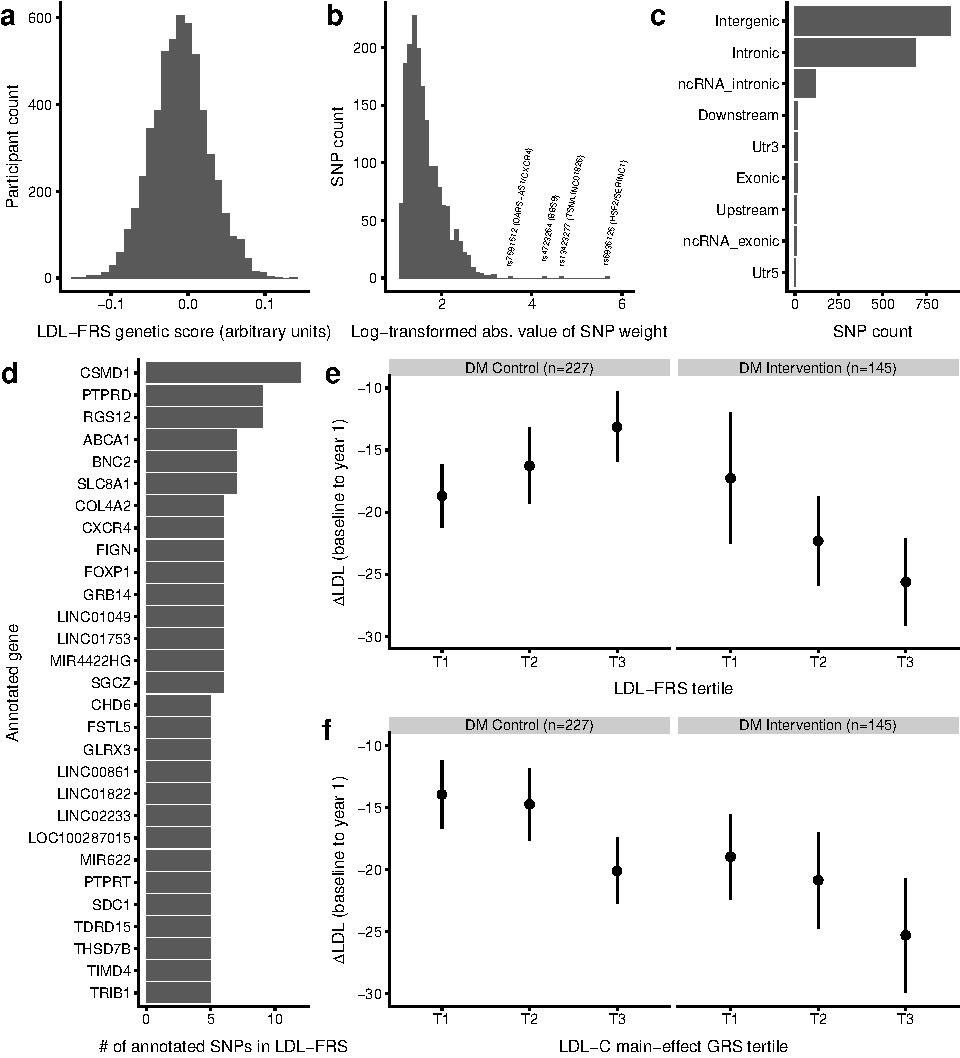
\includegraphics{figures/ldl-score-characterization-1.pdf}
\caption{LDL-FRS characterization. a) Distribution of LDL-FRS in WHI DM
trial participants. b) Distribution of SNP weights constituting the
LDL-FRS (shown as the natural log-transformed absolute values of the
true weights). c) SNP counts in different loci types for LDL-FRS
consituent SNPs. d) Genes are summarized by the number of annotated SNPs
in the LDL-FRS (genes with at least 5 component SNPs are shown). e-f)
1-year changes in LDL-C in DM trial participants as a function of
genetic scores. Mean changes in LDL-C (y-axis) are shown as a function
of either LDL-FRS (e) or LDL-GRS (f) tertile (x-axis). Error bars
represent standard errors. LDL-FRS: LDL-C fat response genetic score,
LDL-GRS: LDL-C main-effect genetic score.}
\end{figure}

Differences in mean LDL-C changes during the DM trial across genetic
score strata are shown in Fig. 1e,f. As suggested by the regression
results, those in the control arm trended towards less strong LDL-C
reductions in higher LDL-FRS strata, while those in the fat-reduction
arm showed the opposite trend. For comparison to the FRS, a main-effect
genetic risk score (GRS) for LDL-C was developed using summary
statistics from the Global Lipid Genetics Consortium meta-analysis
(Willer et al. 2013) and an identical pruning-and-thresholding procedure
to that used for the GDI-based scores. As expected, this score was
strongly predictive of baseline LDL-C concentrations (p=4.53e-27).
However, unlike the GDI-based score, the GRS did not predict LDL-C
changes in the DM intervention group (p=0.15; stratum-specific mean
changes in Fig. 1f).

\hypertarget{ldl-frs-association-with-chronic-disease-outcomes}{%
\subsection{LDL-FRS association with chronic disease
outcomes}\label{ldl-frs-association-with-chronic-disease-outcomes}}

\begin{figure}
\centering
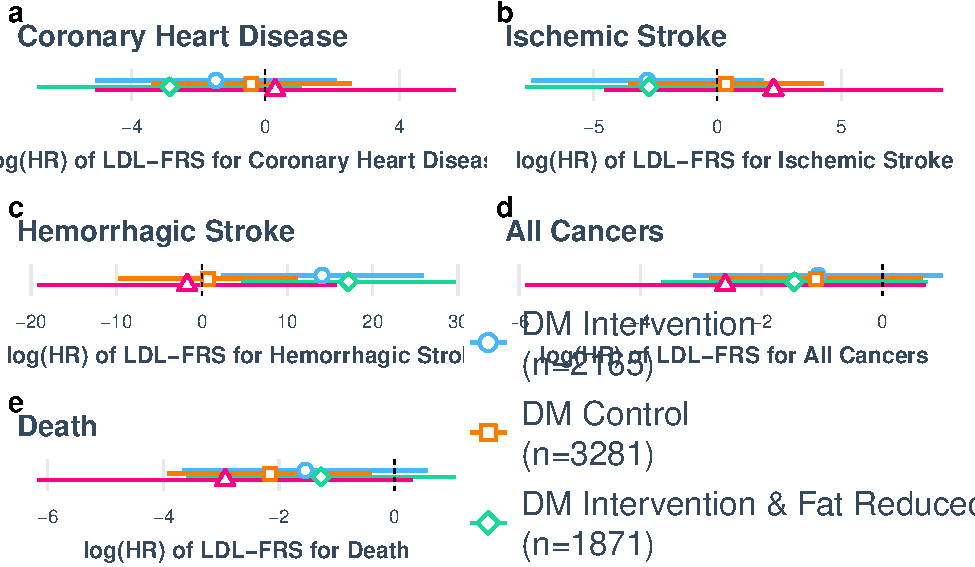
\includegraphics{figures/cvd-outcomes-1.pdf}
\caption{FRS prediction of chronic disease development. X-axis shows
log(hazard ratio) estimates from Cox proportional hazards regression for
a) coronary heart disease, b) myocardial infraction, c) stroke, d)
cancer (any type), and e) death from all causes. Separate estimates are
shown for DM trial intervention arm, control arm, and the same strata
filtered for FFQ-reported fat reduction or increase, respectively. Error
bars represent 95\% confidence interval estimates for the regression
coefficients.}
\end{figure}

Next, the LDL-FRS was tested for relationships with incident disease
outcomes using Cox proportional hazards models adjusted for age at
baseline (Fig. 2). In addition to intervention versus control arm,
another set of ``per protocol-like'' strata were produced by
additionally filtering for FFQ-based self-reported fat reduction (in the
intervention group) or fat increase (in the control group). CHD and
ischemic stroke appeared visually to demonstrate expected interaction
patterns (an inverse association between LDL-FRS and disease risk only
in the fat reduction group), but these estimates contained a high level
of variability. Results for cancer were equivocal and did not vary
across groups. Hemorrhagic stroke showed significant positive
associations with the LDL-FRS only in the fat reduction group.
Additionally, the score associated with a decrease in time-to-death in
fat-increasing strata, those most likely to have undergone a sustained
increase in dietary fat over time.

\hypertarget{discussion}{%
\section{Discussion}\label{discussion}}

Diet response scores have shown some success at predicting the response
of cardiovascular risk factors (CRFs) to nutritional interventions, but
they are often based solely on main effects or single GDI SNPs. Here, we
explored the potential for gene diet interaction (GDI)-based diet
responder score development, leveraging the multi-trial setup of the
Women's Health Initiative. We developed what to our knowledge is the
first example of a diet response score based on a hypothesis-free genome
scan for each of six risk factors, and showed preliminary evidence for
the viability of a LDL-C fat response score.

Though FRS for six CRFs were developed and tested, only that for LDL-C
showed nominal significance in predicting 1-year changes in the
corresponding CRF. Multiple factors could explain this lack of
predictive performance in general. First, analysis in observational
datasets carries with it the potential for confounding of the observed
relationships. Second, FFQs are imprecise instruments for measuring
dietary intake, and though the FFQs used in the present study were
optimized for detection of dietary fat, there was potential for
substantial misclassification of this environmental exposure. Third,
power calculations shown here and elsewhere suggest that a cohort of
this size may not be powered to detect many very small gene-environment
interactions such as are sought in genome-wide approaches like the one
used here.

CSMD1, PTPRD, and RGS12 stood out as genes containing the highest number
of SNPs in the LDL-FRS (11, 9, and 9, respectively, after LD-pruning for
r\textsuperscript{2} \textless{} 0.5. CSMD1 variants are notably
associated with LDL-C response to statin treatment (Thompson et al.
2009) as well as SBP response to a high-salt diet {[}Newton-Cheh2009{]}.
CSMD1 has also shown epigenetic associations with LDL-C (Bell et al.
2012) as well as response to modification of dietary fat composition
(Perfilyev et al. 2017). PTPRD variants modulate the response of T2D
patients to pioglitazone therapy (Pei et al. 2013) and show suggestive
associations with eating behaviors (caloric intake at dinner) (Comuzzie
et al. 2012). RGS12 has been linked to LDL-C in GWAS (Spracklen et al.
2017). Altogether, these genes have literature evidence for
relationships to dietary intake, response to cardiometabolic therapies,
and LDL-C, but have not until now been shown to directly modify the
LDL-C response to dietary fat proportions. We note that there is a bias
towards identifying LDL-C-related variants in the LDL-FRS, as only
nominally-associated main-effect SNPs were used as input to the score
development algorithm.

A reasonable body of literature exists establishing GDIs for both
dietary fat on CRFs (Cuda et al. 2012; Zheng et al. 2015) and general
dietary exposures on LDL-C (Ordovás, Robertson, and Cléirigh 2011).
Multiple studies have looked specifically at genetic variants modulating
the LDL-C response to dietary fat. For example, a caloric restriction
intervention in type 2 diabetics was more effective in reducing LDL-C in
APOE4 carriers (-15.6\% versus -0.7\%) (Saito et al. 2004). Two studies
using the POUNDS LOST trial found relationships of specific
polymorphisms with 2-year changes in response to a dietary fat
intervention. Carriers of a risk allele at the APOA5 variant rs964184
show a decrease of 7.5 mg/dL in LDL-C in low-fat but not high-fat
interventions (Zhang et al. 2012), and carriers of the minor allele at
CETP rs3764261 show an 8.9 mg/dL greater decrease in LDL-C on a low-fat
diet (Xu et al. 2015). Our observed effect size of a 5.4 mg/dL decrease
in LDL-C is of a similar magnitude to these findings, and emerged
despite the multi-factorial nature of the WHI DM trial (which
incorporated additional nutrition recommendations). The observed
variance explained of 3.4\% for the LDL-FRS means that the score, while
contributing meaningfully to the prediction, does not capture most of
the interindividual variability in LDL-C response to the WHI DM trial
intervention.

There has been interest in the past in using main-effect genetic risk
scores (GRS) as genetic variables in order to improve statistical power
to detect gene-environment interactions (Aschard 2016). Such
interactions may be viewed from a lens in which genetic risk corresponds
to a predisposition that is only triggered in certain environments
(e.g.~dietary behaviors). Here, we observed only a minor association of
a main-effect GRS for LDL-C with greater LDL-C reductions in the DM
trial (p=4.5e-27). This trend runs counter to a prior observation of
greater lifestyle intervention effectiveness for LDL-C reduction in
those with low genetic risk of hyperlipidemia (Zubair et al. 2019). This
discrepancy may be due to differences between the DM trial and the
personalized diet and lifestyle changes recommended in the intervention
in question. Regardless, the meaningful increase in predictive power of
the GDI-based FRS compared to the main-effect GRS for LDL-C indicates
the value in using interaction-based scores rather than simple genetic
predispositions for the development of personalized dietary
recommendations.

A diet response score such as that developed here is most useful if its
value extends beyond just risk factor changes and predicts downstream
changes in chronic disease and mortality risk. A modest interaction for
CHD and ischemic stroke was visually apparent across strata (Fig. 2a,b),
corresponding to a decreased CHD risk in fat-reduction participants
whose LDL-C would be expected to drop more prominently according to the
score. In contrast, hemorrhagic stroke showed the opposite trend, with a
positive score-disease relationship only in the fat reduction group.
This result is in line with existing evidence for the detrimental
effects of low LDL-C on hemorrhagic stroke risk (Sun et al. 2019).
Cancer showed no major patterns, which could be expected due to the
equivocal associations of cancer with lipids (Koene et al. 2016).
Somewhat surprisingly, we observed that a fat-response score
predisposing individuals to a positive fat-LDL-C correlation is
inversely associated with risk of death most strongly control
individuals with self-reported fat increases, whose LDL-C would be
expected to rise. However, it is well-appreciated that LDL-C associates
inversely with survival in older populations (Ravnskov et al. 2016) and
this inverse relationship in the control group was not notably different
than that in the intervention group. We note that all disease outcome
relationships assessed here are subject to the major caveat that dietary
evolution and decreased adherence likely developed over time in many
subjects, diluting the utility of the randomization and 1-year changes
used for stratification in Fig. 2.

The present study had the advantage of developing a GDI-based dietary
fat score in almost 10,000 women and testing in a dietary intervention
trial from the same population. However, the sample size did not afford
statistical power to scan genome-wide for GDIs, and the smaller
fractions of alternate ancestries in this population made development of
ancestry-specific response scores unrealistic. Additionally, the DM
trial intervention in which the scores were tested may not exactly match
the intervention relevant to the purely fat reduction-focused score
developed here; it included additional non-fat-related dietary
recommendations that may have effected the interactions examined here,
and did not ultimately achieve its intended 20\% fat reduction. Finally,
this study only examined women, despite the fact that CRF profiles and
their genetic trait architectures are known to vary across sexes.

In summary, we present a method for the development of diet response
scores based on genome-wide gene-diet interaction study summary
statistics. While the resulting dietary fat response scores are not all
informative, a score focused on LDL-C is predictive of 1-year LDL-C
changes during a fat reduction trial. Its performance is risk
factor-specific, and is superior to that of a main-effect genetic risk
score for LDL-C. Furthermore, it displays suggestive relationships with
chronic disease outcomes, adding a new perspective to known
discrepancies between associations of LDL-C with cardiovascular disease,
stroke subtypes, and all-cause mortality. These findings support the
utility of gene-diet interactions for personalized nutrition while
highlighting the need for increased sample sizes and improved diet
measures for the discovery of robust genetic predictors of diet
response.

\hypertarget{methods}{%
\section{Methods}\label{methods}}

\hypertarget{womens-health-initiative-dataset}{%
\subsection{Women's Health Initiative
Dataset}\label{womens-health-initiative-dataset}}

The Women's Health Initiative study consists of a series of substudies:
three clinical trials (related to cancer, cardiovascular disease, and
osteoporosis) and an observational study (Anderson et al. 1998). Over
160,000 participants were enrolled between 1993-1998, with the ability
to enroll in up to 3 of the clinical trials simultaneously. For the
purposes of this analysis, participants were categorized based only on
whether or not they were enrolled in the dietary modification (DM)
trial, which randomized almost 50,000 women to a low-fat diet or a
control diet with no recommended dietary changes, with primary outcomes
being incidence of breast and colorectal cancers and heart disease
{[}Ritenbaugh et al. (2003). Participants were comprehensively screened
at baseline, including physical measurements, blood sample collection,
and questionnaire administration, while only a subset of participants
provided blood samples or returned questionnaires during later visits.
The food frequency questionnaire (FFQ) was designed specifically for the
WHI study, emphasizing specific foods and preparation methods to
maximize its sensitivity to changes in fat intake (Patterson et al.
1999).

Phenotype data were accessed from dbGaP (accession: phs000746.v2.p3).
Values shown in Table 1 only pertain to women whose genotypes were
measured in one of a series of follow-up studies. For gene-diet
interaction analyses, SBP, LDL-C, and GLU were adjusted for medication
use: LDL-C and GLU values were divided by 0.75 for those on
lipid-lowering and anti-diabetic medication, respectively, and SBP
values were increased by 15 mmHg for those on anti-hypertensive
medication. Cardiovascular risk factors (CRFs) were winsorized at 5
standard deviations from the mean and those other than LDL-C (BMI, SBP,
HDL-C, TG, and GLU) were log-transformed prior to analysis. Longitudinal
risk factor changes were calculated in DM trial participants as the
difference between baseline and year 1. Phenotype data processing was
performed using R version 3.4.3 (R Core Team 2017) and Python version
3.6.0.

\hypertarget{genotype-data-and-preprocessing}{%
\subsection{Genotype data and
preprocessing}\label{genotype-data-and-preprocessing}}

Imputed genotype data were retrieved from dbGaP (accession:
phs000746.v2.p3) as a harmonized set of imputation outputs from a series
of genotyping studies involving WHI participants. Prior to imputation,
study-specific quality control steps had been undertaken on
directly-genotyped SNPs, with filters based on sample and call rate,
Hardy-Weinberg equilibrium, and minor allele frequency. Phasing had been
performed for autosomes using BEAGLE, followed by imputation using
minimac (MACH for the SHARe study subset). After download from dbGaP,
variants were filtered for imputation R-squared \textgreater{} 0.3 and
minor allele frequency (MAF) \textgreater{}0.001 and annotated with
rsIDs, loci, and allelic information using the 1000 Genomes Phase 3
download from dbSNP (download date: April 13, 2018). Only variants
passing the imputation quality threshold in all genotyping sub-studies
were included in the final dosage dataset. For score development and
mputed variant dosages were converted to hard-calls and set to missing
if the estimated dosage was not within 0.1 of an integer allele count.
Post-imputation genotype data processing was performed using PLINK 2.0,
while clumping, and score calculation were performed using PLINK 1.9
(Chang et al. 2015).

\hypertarget{genome-wide-interaction-study}{%
\subsection{Genome-wide interaction
study}\label{genome-wide-interaction-study}}

A genome-wide interaction study was performed for each of the six
cardiometabolic risk factors. The genome-wide scan used an additive
genotype model, adjusted for dietary fat (binary: \% of kcals above or
below the median), total kcals per day, age, and five ancestry principal
components. The primary estimand of interest was the interaction term
between dietary fat and minor allele count at the SNP of interest.
Interaction analyses were carried out using PLINK 2.0 (Chang et al.
2015). Variants of interest were annotated to genes using the Annovar
tool (Wang, Li, and Hakonarson 2010).

Gene-environment interaction power calculations for single SNPs were
performed using the Quanto tool (Gauderman 2002). The following
assumptions were made: additive model; variance explained by genotype
alone = 0.5\%; and binary environment with 50\% prevalence and
explaining 10\% of variance. (Note: there is no effect of minor allele
frequency in this case given that variances explained are directly
specified.)

\hypertarget{genetic-responder-score-construction-and-evaluation}{%
\subsection{Genetic responder score construction and
evaluation}\label{genetic-responder-score-construction-and-evaluation}}

To prioritize variants for inclusion in genetic responder scores,
nominal (p\textless{}0.05) variants for main-effect on each risk factor
were retrieved from large-scale meta-analyses: GIANT for BMI (Yengo et
al. 2018); International Consortium for Blood Pressure for SBP (Ehret et
al. 2011); Global Lipid Genetics Consortium (GLGC) for LDL-C, HDL-C, and
TG (Willer et al. 2013); and MAGIC for fasting glucose (Dupuis et al.
2010). Each FRS was constructed using summary statistics for the
diet-SNP interaction terms from the associated GWIS. SNPs were filtered
for nominal main-effect relationships using the above meta-analyses, and
interaction summary statistics were used as input to a
pruning-and-thresholding (P\&T) procedure (using the ``--clump''
function in PLINK 1.9), with a seed threshold of p=0.05 and an LD
threshold of r\textsuperscript{2}=0.5. The linkage disequilibrium
references for the procedure was calculated from genotypes of the white
DM trial participants. Genetic fat response scores (FRS) for each
individual were then calculated as the weighted sum of allelic dosages
for variants selected by the P\&T procedure, with weights corresponding
to the GWIS interaction term estimates. A genetic risk score for LDL-C
was created using the GLGC LDL-C meta-analysis summary statistics and
the same P\&T method and parameters as was used for the interaction
analyses, resulting in a 26467-SNP score.

FRS were used to test for discrimination of changes in CRFs over the
first year of the DM trial. Risk factor changes were assessed using
linear models in participants in the intervention arm, with and without
adjustment for baseline CRF levels. As a sensitivity analysis, p-values
were calculated in separate models for interaction of the genetic score
with 1) trial arm (control vs.~dietary modification), and 2) observed
fat reduction (negative vs.~positive 3-year change in FFQ-estimated
dietary fat). GRS were further tested for prediction of chronic disease
development during follow-up across DM trial strata. Time-to-event for
each of coronary heart disease, myocardial infarction, stroke, cancer,
and death were collected and used to fit age-adjusted Cox proportional
hazards models. Estimated log-hazard ratios were extracted from
regressions conducted in the following strata: 1) DM trial intervention
arm, 2) DM trial control arm, 3) DM trial intervention arm filtered for
participants with 1-year fat reduction based on FFQ, and 4) DM trial
control arm filtered for participants with 1-year fat increase based on
FFQ.

\hypertarget{supplementary-data}{%
\section{Supplementary Data}\label{supplementary-data}}

\newcommand{\beginsupplement}{%
        \setcounter{table}{0}
        \renewcommand{\thetable}{S\arabic{table}}%
        \setcounter{figure}{0}
        \renewcommand{\thefigure}{S\arabic{figure}}%
     }
%
        \setcounter{table}{0}
        \renewcommand{\thetable}{S\arabic{table}}%
        \setcounter{figure}{0}
        \renewcommand{\thefigure}{S\arabic{figure}}%

\begin{longtable}{rrrr}
\caption{\label{tab:show-power-calcs}Sample size necessary to achieve power of 0.8}\\
\toprule
GxE variance explained (\%) & N (nominal) & N (suggestive) & N (genome-wide)\\
\midrule
0.05 & 14046 & 49488 & 70866\\
0.10 & 7021 & 24737 & 35423\\
0.50 & 1401 & 4936 & 7069\\
1.00 & 699 & 2461 & 3524\\
\bottomrule
\end{longtable}

\begin{figure}
\centering
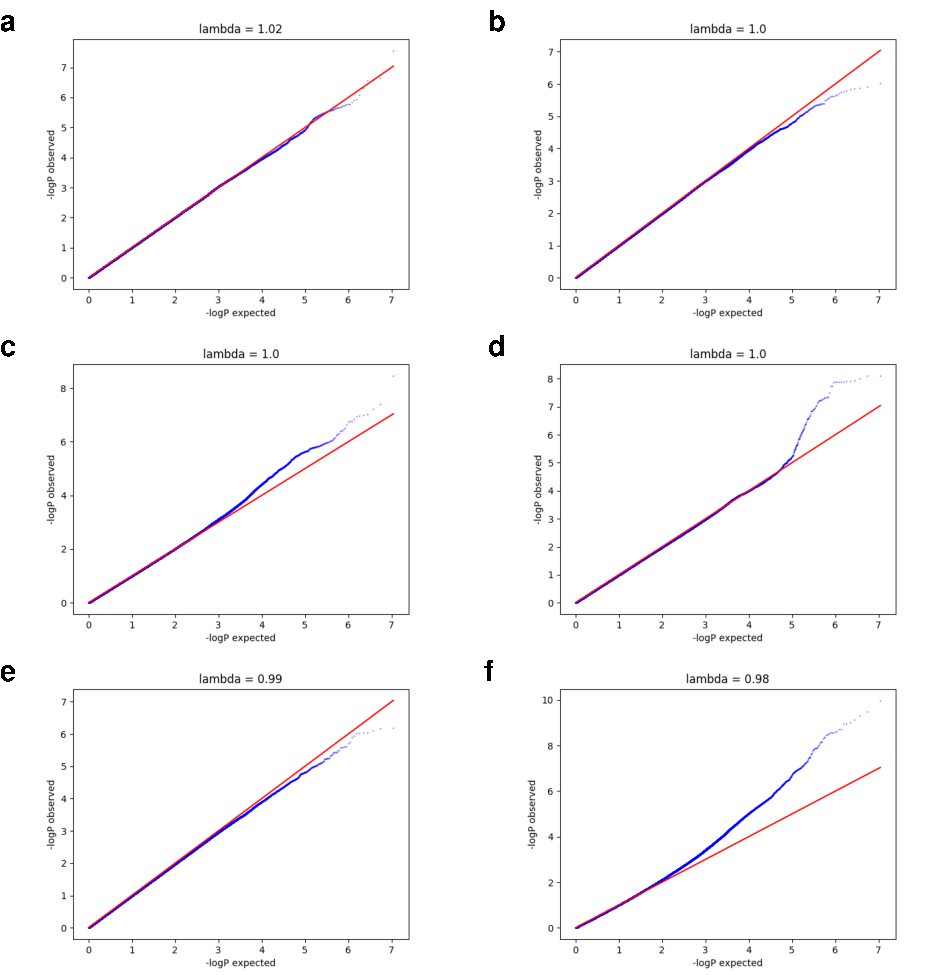
\includegraphics{figures/show-qq-plots-1.pdf}
\caption{Q-Q plots from individual CRF GWIS. The distribution of
p-values from each GWIS is plotted against the expected uniform p-value
distribution. Plots correspond to: a) BMI, b) SBP, c) LDL-C, d) HDL-C,
e) TG, and f) FG.}
\end{figure}

\begin{longtable}{llllllllll}
\caption{\label{tab:show-test-scores-cross-ancestry}Responder score effects on CRF changes in DM trial participants across ancestries}\\
\toprule
\multicolumn{1}{c}{} & \multicolumn{3}{c}{All combined} & \multicolumn{3}{c}{Black} & \multicolumn{3}{c}{Hispanic} \\
\cmidrule(l{3pt}r{3pt}){2-4} \cmidrule(l{3pt}r{3pt}){5-7} \cmidrule(l{3pt}r{3pt}){8-10}
CRF & N & Std. effect size & P-value & N & Std. effect size & P-value & N & Std. effect size & P-value\\
\midrule
BMI & 3606 & -0.02 & 0.24 & 1214 & 0 & 0.994 & 404 & 0.018 & 0.719\\
FG & 572 & 0.08 & 0.043 & 214 & -0.004 & 0.955 & 77 & -0.014 & 0.901\\
HDL-C & 430 & -0.06 & 0.224 & 206 & -0.096 & 0.182 & 74 & -0.057 & 0.66\\
LDL-C & 422 & 0.084 & 0.066 & 206 & 0.055 & 0.412 & 71 & 0.126 & 0.227\\
SBP & 3645 & 0.041 & 0.015 & 1230 & 0 & 0.991 & 411 & -0.008 & 0.868\\
\addlinespace
TG & 430 & -0.075 & 0.112 & 206 & -0.023 & 0.743 & 74 & -0.098 & 0.433\\
\bottomrule
\end{longtable}

\begin{ThreePartTable}
\begin{TableNotes}
\item * Std. effect size represents the regression coefficient estimate in terms of CRF standard deviation per responder score standard deviation
\end{TableNotes}
\begin{longtable}{lrrrr}
\caption{\label{tab:show-test-ldl-scores-other-rfs}LDL-FRS effects on alternate CRF changes in DM trial participants}\\
\toprule
Outcome risk factor & \# SNPs in risk score & Sample size & Std. effect size & P-value\\
\midrule
BMI & 1747 & 1988 & -0.02 & 0.36\\
SBP & 1747 & 2004 & 0.00 & 0.83\\
HDL-C & 1747 & 150 & -0.07 & 0.39\\
TG & 1747 & 150 & 0.11 & 0.16\\
FG & 1747 & 281 & 0.01 & 0.82\\
\bottomrule
\insertTableNotes
\end{longtable}
\end{ThreePartTable}

\hypertarget{references}{%
\section*{References}\label{references}}
\addcontentsline{toc}{section}{References}

\hypertarget{refs}{}
\leavevmode\hypertarget{ref-Anderson1998}{}%
Anderson, Garnet L, Steven R Cummings, Laurence S Freedman, Curt
Furberg, Maureen M Henderson, Susan R Johnson, Lewis H Kuller, et al.
1998. ``Design of the Women's Health Initiative Clinical Trial and
Observational Study.'' \emph{Controlled Clinical Trials} 19 (1):
61--109. \url{https://doi.org/10.1016/S0197-2456(97)00078-0}.

\leavevmode\hypertarget{ref-Aschard2016}{}%
Aschard, Hugues. 2016. ``A perspective on interaction effects in genetic
association studies.'' \emph{Genetic Epidemiology} 40 (8): 678--88.
\url{https://doi.org/10.1002/gepi.21989}.

\leavevmode\hypertarget{ref-Bell2012}{}%
Bell, Jordana T., Pei-Chien Tsai, Tsun-Po Yang, Ruth Pidsley, James
Nisbet, Daniel Glass, Massimo Mangino, et al. 2012. ``Epigenome-Wide
Scans Identify Differentially Methylated Regions for Age and Age-Related
Phenotypes in a Healthy Ageing Population.'' Edited by Jun Li.
\emph{PLoS Genetics} 8 (4): e1002629.
\url{https://doi.org/10.1371/journal.pgen.1002629}.

\leavevmode\hypertarget{ref-Chang2015}{}%
Chang, Christopher C., Carson C. Chow, Laurent C.A.M. Tellier, Shashaank
Vattikuti, Shaun M. Purcell, and James J. Lee. 2015. ``Second-generation
PLINK: rising to the challenge of larger and richer datasets.''
\emph{GigaScience} 4 (1): 7.
\url{https://doi.org/10.1186/s13742-015-0047-8}.

\leavevmode\hypertarget{ref-Comuzzie2012}{}%
Comuzzie, Anthony G, Shelley A Cole, Sandra L Laston, V Saroja
Voruganti, Karin Haack, Richard A Gibbs, and Nancy F Butte. 2012.
``Novel Genetic Loci Identified for the Pathophysiology of Childhood
Obesity in the Hispanic Population.'' Edited by Dana C. Crawford.
\emph{PLoS ONE} 7 (12): e51954.
\url{https://doi.org/10.1371/journal.pone.0051954}.

\leavevmode\hypertarget{ref-Corella2013}{}%
Corella, D., P. Carrasco, J. V. Sorli, R. Estruch, J. Rico-Sanz, M. A.
Martinez-Gonzalez, J. Salas-Salvado, et al. 2013. ``Mediterranean Diet
Reduces the Adverse Effect of the TCF7L2-rs7903146 Polymorphism on
Cardiovascular Risk Factors and Stroke Incidence: A randomized
controlled trial in a high-cardiovascular-risk population.''
\emph{Diabetes Care}, dc13--0955 --.
\url{https://doi.org/10.2337/dc13-0955}.

\leavevmode\hypertarget{ref-Corella2009}{}%
Corella, Dolores, Gina Peloso, Donna K. Arnett, Serkalem Demissie, L.
Adrienne Cupples, Katherine Tucker, Chao Qiang Lai, et al. 2009.
``APOA2, dietary fat, and body mass index: Replication of a gene-diet
interaction in 3 independent populations.'' \emph{Archives of Internal
Medicine}. \url{https://doi.org/10.1001/archinternmed.2009.343}.

\leavevmode\hypertarget{ref-Cornelis2006}{}%
Cornelis, Marilyn C., Ahmed El-Sohemy, Edmond K. Kabagambe, and Hannia
Campos. 2006. ``Coffee, CYP1A2 genotype, and risk of myocardial
infarction.'' \emph{Journal of the American Medical Association}.
\url{https://doi.org/10.1001/jama.295.10.1135}.

\leavevmode\hypertarget{ref-Cuda2011}{}%
Cuda, Cristina, Alaa Badawi, Mohamed Karmali, and Ahmed El-Sohemy. 2011.
``Polymorphisms in Toll-like receptor 4 are associated with factors of
the metabolic syndrome and modify the association between dietary
saturated fat and fasting high-density lipoprotein cholesterol.''
\emph{Metabolism} 60 (8): 1131--5.
\url{https://doi.org/10.1016/j.metabol.2010.12.006}.

\leavevmode\hypertarget{ref-Cuda2012}{}%
Cuda, Cristina, Bibiana Garcia-Bailo, Mohamed Karmali, Ahmed El-Sohemy,
and Alaa Badawi. 2012. ``A common polymorphism near the interleukin-6
gene modifies the association between dietary fat intake and insulin
sensitivity.'' \emph{Journal of Inflammation Research}.
\url{https://doi.org/10.2147/JIR.S27911}.

\leavevmode\hypertarget{ref-Dempfle2008}{}%
Dempfle, Astrid, André Scherag, Rebecca Hein, Lars Beckmann, Jenny
Chang-Claude, and Helmut Schäfer. 2008. ``Gene-environment interactions
for complex traits: Definitions, methodological requirements and
challenges.'' \url{https://doi.org/10.1038/ejhg.2008.106}.

\leavevmode\hypertarget{ref-Dupuis2010}{}%
Dupuis, Josée, Claudia Langenberg, Inga Prokopenko, Richa Saxena, Nicole
Soranzo, Anne U. Jackson, Eleanor Wheeler, et al. 2010. ``New genetic
loci implicated in fasting glucose homeostasis and their impact on type
2 diabetes risk.'' \emph{Nature Genetics}.
\url{https://doi.org/10.1038/ng.520}.

\leavevmode\hypertarget{ref-Ehret2011}{}%
Ehret, Georg B., Patricia B. Munroe, Kenneth M. Rice, Murielle Bochud,
Andrew D. Johnson, Daniel I. Chasman, Albert V. Smith, et al. 2011.
``Genetic variants in novel pathways influence blood pressure and
cardiovascular disease risk.'' \emph{Nature} 478 (7367): 103--9.
\url{https://doi.org/10.1038/nature10405}.

\leavevmode\hypertarget{ref-Figueiredo2014}{}%
Figueiredo, Jane C., Li Hsu, Carolyn M. Hutter, Yi Lin, Peter T.
Campbell, John A. Baron, Sonja I. Berndt, et al. 2014. ``Genome-Wide
Diet-Gene Interaction Analyses for Risk of Colorectal Cancer.''
\emph{PLoS Genetics}.
\url{https://doi.org/10.1371/journal.pgen.1004228}.

\leavevmode\hypertarget{ref-Gauderman2002}{}%
Gauderman, W. J. 2002. ``Sample Size Requirements for Association
Studies of Gene-Gene Interaction.'' \emph{American Journal of
Epidemiology} 155 (5): 478--84.
\url{https://doi.org/10.1093/aje/155.5.478}.

\leavevmode\hypertarget{ref-Huang2015}{}%
Huang, Tao, Jinyan Huang, Qibin Qi, Yanping Li, George A. Bray, Jennifer
Rood, Frank M. Sacks, and Lu Qi. 2015. ``PCSK7 Genotype Modifies Effect
of a Weight-Loss Diet on 2-Year Changes of Insulin Resistance: The
POUNDS LOST Trial.'' \emph{Diabetes Care} 38 (3): 439--44.
\url{https://doi.org/10.2337/dc14-0473}.

\leavevmode\hypertarget{ref-Koene2016}{}%
Koene, Ryan J, Anna E Prizment, Anne Blaes, and Suma H Konety. 2016.
``Shared Risk Factors in Cardiovascular Disease and Cancer.''
\emph{Circulation} 133 (11): 1104--14.
\url{https://doi.org/10.1161/CIRCULATIONAHA.115.020406}.

\leavevmode\hypertarget{ref-Ma2011}{}%
Ma, Q., and A. Y. H. Lu. 2011. ``Pharmacogenetics, Pharmacogenomics, and
Individualized Medicine.'' \emph{Pharmacological Reviews} 63 (2):
437--59. \url{https://doi.org/10.1124/pr.110.003533}.

\leavevmode\hypertarget{ref-Olsen2016}{}%
Olsen, Nanna J., Lars Ängquist, Sofus C. Larsen, Allan Linneberg, Tea
Skaaby, Lise Lotte N. Husemoen, Ulla Toft, et al. 2016. ``Interactions
between genetic variants associated with adiposity traits and soft
drinks in relation to longitudinal changes in body weight and waist
circumference.'' \emph{The American Journal of Clinical Nutrition} 104
(3): 816--26. \url{https://doi.org/10.3945/ajcn.115.122820}.

\leavevmode\hypertarget{ref-Ordovas2018}{}%
Ordovas, Jose M., Lynnette R. Ferguson, E. Shyong Tai, and John C.
Mathers. 2018. ``Personalised nutrition and health.'' \emph{BMJ}, June,
bmj.k2173. \url{https://doi.org/10.1136/bmj.k2173}.

\leavevmode\hypertarget{ref-Ordovas2011}{}%
Ordovás, José M., Ruairi Robertson, and Ellen Ní Cléirigh. 2011.
``Gene--gene and gene--environment interactions defining lipid-related
traits.'' \emph{Current Opinion in Lipidology} 22 (2): 129--36.
\url{https://doi.org/10.1097/MOL.0b013e32834477a9}.

\leavevmode\hypertarget{ref-Patterson1999}{}%
Patterson, Ruth E., Alan R. Kristal, Lesley Fels Tinker, Rachel A.
Carter, Mary Pat Bolton, and Tanya Agurs-Collins. 1999. ``Measurement
Characteristics of the Women's Health Initiative Food Frequency
Questionnaire.'' \emph{Annals of Epidemiology} 9 (3): 178--87.
\url{https://doi.org/10.1016/S1047-2797(98)00055-6}.

\leavevmode\hypertarget{ref-Pei2013}{}%
Pei, Qi, Qiong Huang, Guo-ping Yang, Ying-chun Zhao, Ji-ye Yin, Min
Song, Yi Zheng, Zhao-hui Mo, Hong-hao Zhou, and Zhao-qian Liu. 2013.
``PPAR-\(\gamma\)2 and PTPRD gene polymorphisms influence type 2
diabetes patients' response to pioglitazone in China.'' \emph{Acta
Pharmacologica Sinica} 34 (2): 255--61.
\url{https://doi.org/10.1038/aps.2012.144}.

\leavevmode\hypertarget{ref-Perfilyev2017}{}%
Perfilyev, Alexander, Ingrid Dahlman, Linn Gillberg, Fredrik Rosqvist,
David Iggman, Petr Volkov, Emma Nilsson, Ulf Risérus, and Charlotte
Ling. 2017. ``Impact of polyunsaturated and saturated fat overfeeding on
the DNA-methylation pattern in human adipose tissue: a randomized
controlled trial.'' \emph{The American Journal of Clinical Nutrition}
105 (4). American Society for Nutrition: 991--1000.
\url{https://doi.org/10.3945/ajcn.116.143164}.

\leavevmode\hypertarget{ref-Qi2012}{}%
Qi, Qibin, Audrey Y. Chu, Jae H. Kang, Majken K. Jensen, Gary C. Curhan,
Louis R. Pasquale, Paul M. Ridker, et al. 2012. ``Sugar-Sweetened
Beverages and Genetic Risk of Obesity.'' \emph{New England Journal of
Medicine} 367 (15): 1387--96.
\url{https://doi.org/10.1056/NEJMoa1203039}.

\leavevmode\hypertarget{ref-Ravnskov2016}{}%
Ravnskov, Uffe, David M. Diamond, Rokura Hama, Tomohito Hamazaki, Björn
Hammarskjöld, Niamh Hynes, Malcolm Kendrick, et al. 2016. ``Lack of an
association or an inverse association between low-density-lipoprotein
cholesterol and mortality in the elderly: a systematic review.''
\emph{BMJ Open} 6 (6): e010401.
\url{https://doi.org/10.1136/bmjopen-2015-010401}.

\leavevmode\hypertarget{ref-RCoreTeam2017}{}%
R Core Team. 2017. ``R: A language and environment for statistical
computing.'' Vienna, Austria: R Foundation for Statistical Computing.
\url{https://www.r-project.org/}.

\leavevmode\hypertarget{ref-Ritenbaugh2003}{}%
Ritenbaugh, Cheryl, Ruth E Patterson, Rowan T Chlebowski, Bette Caan,
Lesley Fels-Tinker, Barbara Howard, and Judy Ockene. 2003. ``The women's
health initiative dietary modification trial: overview and baseline
characteristics of participants.'' \emph{Annals of Epidemiology}.
\url{https://doi.org/10.1016/s1047-2797(03)00044-9}.

\leavevmode\hypertarget{ref-Saito2004}{}%
Saito, Mieko, Masaaki Eto, Hayami Nitta, Yukiko Kanda, Makoto Shigeto,
Katsura Nakayama, Kazuhito Tawaramoto, et al. 2004. ``Effect of
Apolipoprotein E4 Allele on Plasma LDL Cholesterol Response to Diet
Therapy in Type 2 Diabetic Patients.'' \emph{Diabetes Care} 27 (6):
1276--80. \url{https://doi.org/10.2337/diacare.27.6.1276}.

\leavevmode\hypertarget{ref-Smith2018}{}%
Smith, Caren E., Jack L. Follis, Hassan S. Dashti, Toshiko Tanaka,
Mariaelisa Graff, Amanda M. Fretts, Tuomas O. Kilpeläinen, et al. 2018.
``Genome-Wide Interactions with Dairy Intake for Body Mass Index in
Adults of European Descent.'' \emph{Molecular Nutrition and Food
Research}. \url{https://doi.org/10.1002/mnfr.201700347}.

\leavevmode\hypertarget{ref-Spracklen2017}{}%
Spracklen, Cassandra N., Peng Chen, Young Jin Kim, Xu Wang, Hui Cai,
Shengxu Li, Jirong Long, et al. 2017. ``Association analyses of East
Asian individuals and trans-ancestry analyses with European individuals
reveal new loci associated with cholesterol and triglyceride levels.''
\emph{Human Molecular Genetics} 26 (9): 1770--84.
\url{https://doi.org/10.1093/hmg/ddx062}.

\leavevmode\hypertarget{ref-Sun2019}{}%
Sun, Luanluan, Robert Clarke, Derrick Bennett, Yu Guo, Robin G. Walters,
Michael Hill, Sarah Parish, et al. 2019. ``Causal associations of blood
lipids with risk of ischemic stroke and intracerebral hemorrhage in
Chinese adults.'' \url{https://doi.org/10.1038/s41591-019-0366-x}.

\leavevmode\hypertarget{ref-Thompson2009}{}%
Thompson, John F., Craig L. Hyde, Linda S. Wood, Sara A. Paciga, David
A. Hinds, David R. Cox, G. Kees Hovingh, and John J.P. Kastelein. 2009.
``Comprehensive Whole-Genome and Candidate Gene Analysis for Response to
Statin Therapy in the Treating to New Targets (TNT) Cohort.''
\emph{Circulation: Cardiovascular Genetics} 2 (2): 173--81.
\url{https://doi.org/10.1161/CIRCGENETICS.108.818062}.

\leavevmode\hypertarget{ref-Wang2010}{}%
Wang, Kai, Mingyao Li, and Hakon Hakonarson. 2010. ``ANNOVAR: functional
annotation of genetic variants from high-throughput sequencing data.''
\emph{Nucleic Acids Research} 38 (16): e164--e164.
\url{https://doi.org/10.1093/nar/gkq603}.

\leavevmode\hypertarget{ref-Willer2013}{}%
Willer, Cristen J., Ellen M. Schmidt, Sebanti Sengupta, Gina M. Peloso,
Stefan Gustafsson, Stavroula Kanoni, Andrea Ganna, et al. 2013.
``Discovery and refinement of loci associated with lipid levels.''
\emph{Nature Genetics} 45 (11): 1274--83.
\url{https://doi.org/10.1038/ng.2797}.

\leavevmode\hypertarget{ref-Xu2015}{}%
Xu, Min, San San Ng, George A Bray, Donna H Ryan, Frank M Sacks, Guang
Ning, and Lu Qi. 2015. ``Dietary Fat Intake Modifies the Effect of a
Common Variant in the LIPC Gene on Changes in Serum Lipid Concentrations
during a Long-Term Weight-Loss Intervention Trial.'' \emph{The Journal
of Nutrition} 145 (6): 1289--94.
\url{https://doi.org/10.3945/jn.115.212514}.

\leavevmode\hypertarget{ref-Yengo2018}{}%
Yengo, Loic, Julia Sidorenko, Kathryn E. Kemper, Zhili Zheng, Andrew R.
Wood, Michael N. Weedon, Timothy M. Frayling, Joel Hirschhorn, Jian
Yang, and Peter M. Visscher. 2018. ``Meta-analysis of genome-wide
association studies for height and body mass index in 700000 individuals
of European ancestry.'' \emph{Human Molecular Genetics} 27 (20):
3641--9. \url{https://doi.org/10.1093/hmg/ddy271}.

\leavevmode\hypertarget{ref-Zhang2012}{}%
Zhang, Xiaomin, Qibin Qi, George A. Bray, Frank B. Hu, Frank M. Sacks,
and Lu Qi. 2012. ``APOA5 genotype modulates 2-y changes in lipid profile
in response to weight-loss diet intervention: the Pounds Lost Trial.''
\emph{The American Journal of Clinical Nutrition} 96 (4): 917--22.
\url{https://doi.org/10.3945/ajcn.112.040907}.

\leavevmode\hypertarget{ref-Zheng2015}{}%
Zheng, Yan, Tao Huang, Xiaomin Zhang, Jennifer Rood, George A Bray,
Frank M Sacks, and Lu Qi. 2015. ``Dietary Fat Modifies the Effects of
FTO Genotype on Changes in Insulin Sensitivity.'' \emph{The Journal of
Nutrition} 145 (5): 977--82.
\url{https://doi.org/10.3945/jn.115.210005}.

\leavevmode\hypertarget{ref-Zubair2019}{}%
Zubair, Niha, Matthew P. Conomos, Leroy Hood, Gilbert S. Omenn, Nathan
D. Price, Bonnie J. Spring, Andrew T. Magis, and Jennifer C. Lovejoy.
2019. ``Genetic Predisposition Impacts Clinical Changes in a Lifestyle
Coaching Program.'' \emph{Scientific Reports} 9 (1): 6805.
\url{https://doi.org/10.1038/s41598-019-43058-0}.


\end{document}
